\newpage
\chapter{Krátké shrnutí možností hardware}
Můj software je psaný pro stavebnici BlackBox, která byla vytvořená Tomášem Vavrincem. 
Aktuální verze hardware (v1.1) obsahuje následující funkční bloky:

\begin{figure}
    \begin{small}
        \begin{center}
            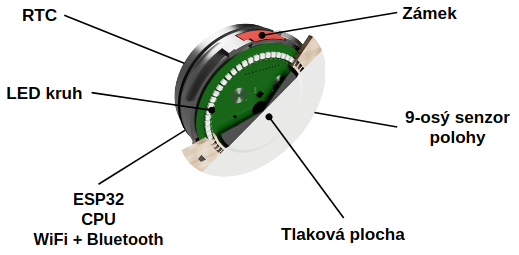
\includegraphics[width=0.95\textwidth]{img/hardware.png}
        \end{center}
        \caption{Hardware}
        \label{fig:hardware}
    \end{small}
\end{figure}

\begin{itemize}[noitemsep]
    \item Hlavní řídící modul
        \begin{itemize}[noitemsep]
            \item ESP32 včetně Wi-fi a bluetooth
            \item Real Time Clock
        \end{itemize}
    \item Uživatelské rozhraní
          \begin{itemize}[noitemsep]
              \item Touchpad
              \item LED kruh
          \end{itemize}
    \item Zámek
        \begin{itemize}[noitemsep]
            \item Motor
            \item Enkodér
            \item IR přijímač
            \item IR vysílač
            \item Zámek sériové linky
        \end{itemize}
    \item Senzory prostředí
          \begin{itemize}[noitemsep]
              \item Magnetometr
              \item Akcelerometr
              \item Gyroskop
              \item Barometr
          \end{itemize}
\end{itemize}

\newpage
\section{Hlavní řídící modul}
Hlavní řídící modul slouží jako výpočetní a~řídící centrum celé desky.

\subsection{ESP32}
BlackBox používá ESP32-WROVER jako svůj procesor.
Základní informace:
\begin{itemize}
    \item Dual core
    \item 240~MHz
    \item 4MB flash
    \item 8MB PSRAM
    \item WiFi, Bluetooth
\end{itemize}

\subsection{Real Time Clock}
Kvůli snížení spotřeby energie bylo implementováno několik mechanismů
Jeden z~těchto mechanismů je i~vypínání všech nepotřebných periferií a~uspání ESP32.V~takovém případě ale není možné uchovat aktuální čas, proto byl na BlackBox přidán modul RTC, ten je napájen přímo z~baterií a~není tak závislý na zbytku BlackBoxu.

\section{Uživatelské rozhraní}

\subsection{Touchpad}
Touchpad je postavený na čipu LDC1614 a jeho alternativách.\footnote{Použitelné jsou pouze alternativy se 4~kanály t.j.~ty, co mají tvar názvu LDCXX14}
Pro měření stisku se využívá deformace kovové destičky a~indukčního měření její vzdálenosti od 4~plošných cívek.
\fxnote{Tady se dá potenciálně napsat spousta věcí :D}

\subsection{LED kruh}
Kruh sestává z~60~adresovatelných RGB LED diod typu WS2812B.

\section{Zámek}

\subsection{Motor a~Encodér}
Zamykací mechanismus je sestaven tak, aby šel BlackBox zasunout do zad trezoru i~v zamčeném stavu, obejde se tedy bez kontroly toho, jestli je při zamykání zasunutý nebo ne.

\subsection{IR komunikace}
IR komunikace je zde obsažená hlavně kvůli synchronizaci se zády trezoru, přesněji k~identifikaci, do kterých zad je BlackBox zasunut.
Tato identifikace by se potenciálně dala dělat pomocí senzorů prostředí, ale za účelem jednoduchosti a~redundance byla zvolena tato možnost.

\subsection{Zámek sériové linky}
Tento mechanismus byl navrhnut za účelem ochrany BlackBox proti neautorizovanému přepsání softwaru.

\section{Senzory prostředí}

\subsection{Senzory polohy}
Tato sada senzorů (akcelerometr, gyroskop, magnetometr) je na různých verzích desky realizována různým způsobem, na verzi 1.0~je realizována jedním čipem obsahujícím všechny tři senzory, ale na verzi 1.1~je realizována pomocí dvou čipů (akcelerometr + gyroskop a~magnetometr)\footnote{Verze 1.1~je zpětně kompatibilní, takže se na ni dá osadit i~čip z~verze 1.0, toho je však v~době psaní této práce nedostatek a~proto byl nahrazen na verzi 1.1 dvěma běžnějšími čipy.}.
Knihovna však musí podporovat všechny možnosti.
Tyto senzory zjišťují natočení BlackBoxu v~prostoru v~9ti osách.
Do budoucna se chystá rozšíření o~GPS senzor.

\subsection{Barometr}
Barometr zde slouží hlavně k hrubému měření výšky, na které se BlackBox nachází.
Případně se také dá použít jako primitivní způsob předpovědi počasí.